\section{Auswertung}
\label{sec:Auswertung}
Aufgrund der zahlreichen Messwerte kann man die zeitlichen Temperaturverläufe sehr genau darstellen.
In den beiden folgenden Abbildungen sind die Temperaturunterschiede der äußeren Sensoren von Messing(breit)[T1], Messing(schmal)[T4] sowie Aluminium[T5] und Edelstahl[T8] gegenübergestellt.
\begin{figure}
    \centering
    \begin{minipage}{.5\textwidth}
        \centering
        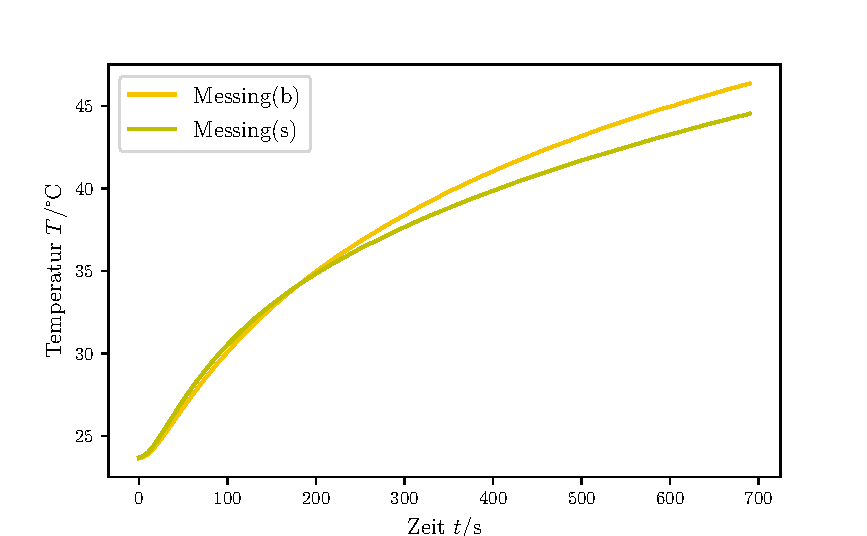
\includegraphics[max width=1.1\linewidth]{build/plot_t1_t4.pdf}
        \caption{T1, T4}
        \label{fig:plot_t1_t4}
    \end{minipage}%
    \begin{minipage}{.5\textwidth}
        \centering
        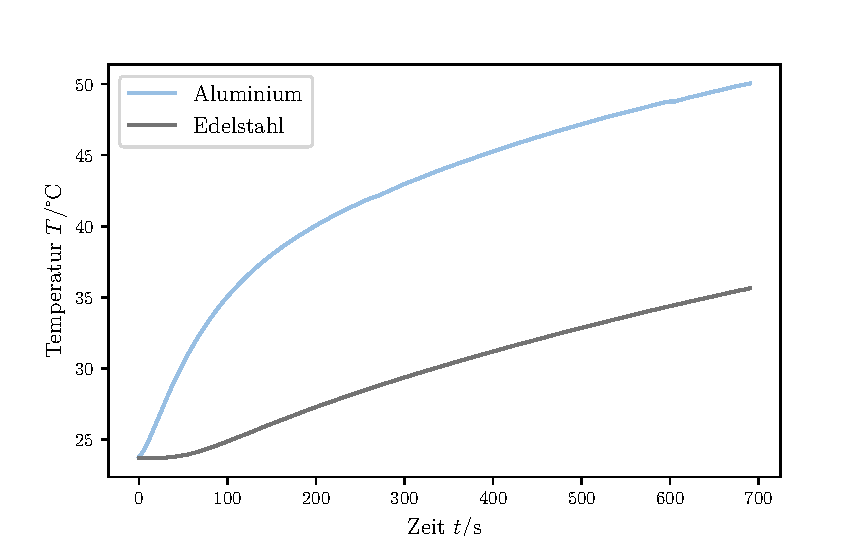
\includegraphics[max width=1.1\linewidth]{build/plot_t5_t8.pdf}
        \caption{T5, T8}
        \label{fig:plot_t5_t8}
    \end{minipage}
    \caption{Zeitliche Temperaturverläufe außen}
    \label{fig:tempDiff_t1t4t5t8}
\end{figure}

\begin{figure}
    \centering
    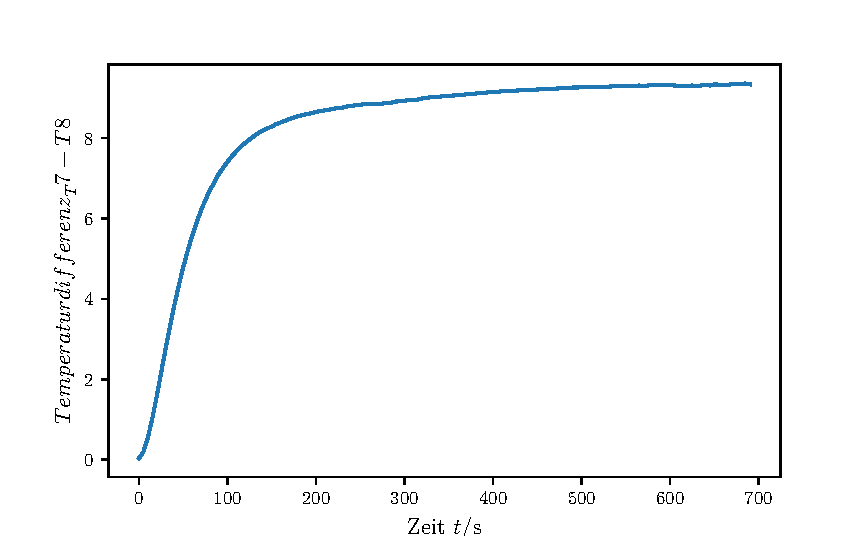
\includegraphics[max width=\linewidth]{build/plot_tempDiff_t7t8.pdf}
    \caption{Erste Messung, statisch.}
    \label{fig:plot_tempDiff_t7t8}
\end{figure}

\begin{figure}
    \centering
    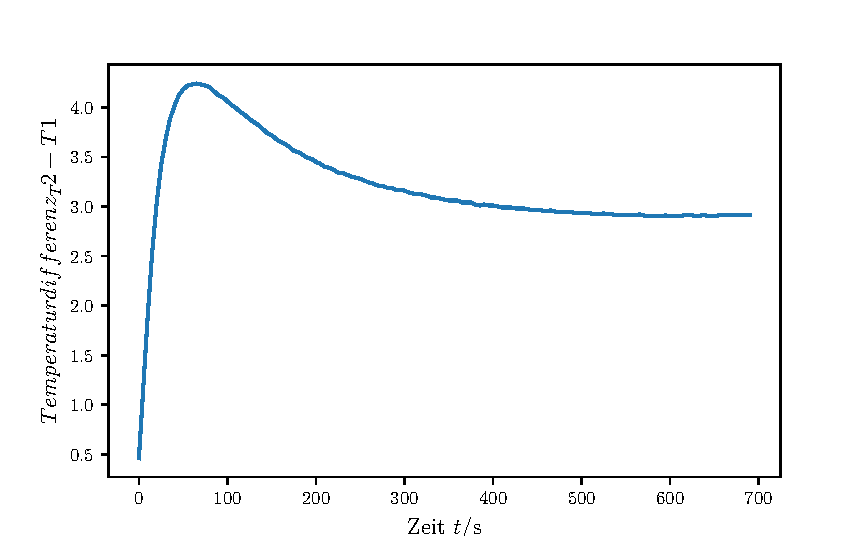
\includegraphics[max width=\linewidth]{build/plot_tempDiff_t2t1.pdf}
    \caption{Erste Messung, statisch.}
    \label{fig:plot_tempDiff_t2t1}
\end{figure}

% \begin{figure}
%     \centering
%     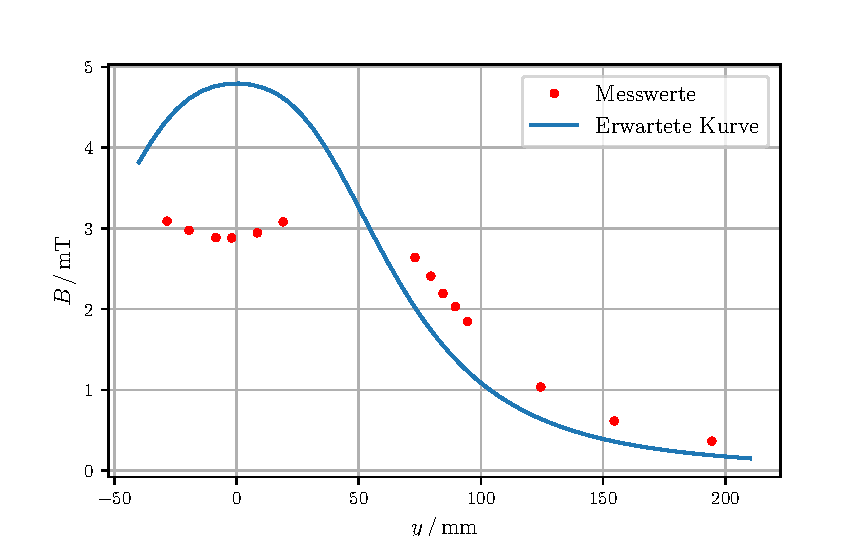
\includegraphics[max width=\linewidth]{plot2.pdf}
%     \caption{Zweite Messung, dynamisch.}
%     \label{fig:plot2}
% \end{figure}

% \begin{figure}
%     \centering
%     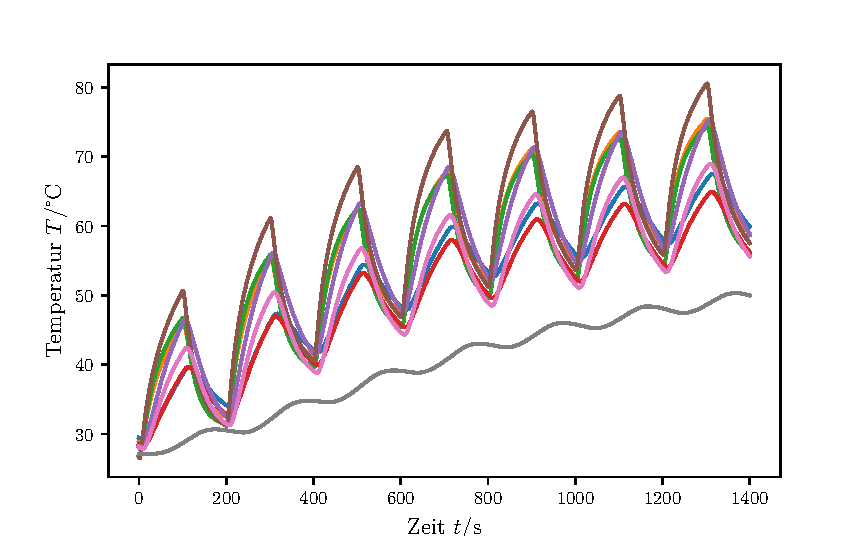
\includegraphics[max width=\linewidth]{plot3.pdf}
%     \caption{Dritte Mesuung, dynamisch - Angström.}
%     \label{fig:plot3}
% \end{figure}